\documentclass[border=10pt]{standalone}
\usepackage{pgfplots}
\pgfplotsset{compat=1.18}
\begin{document}
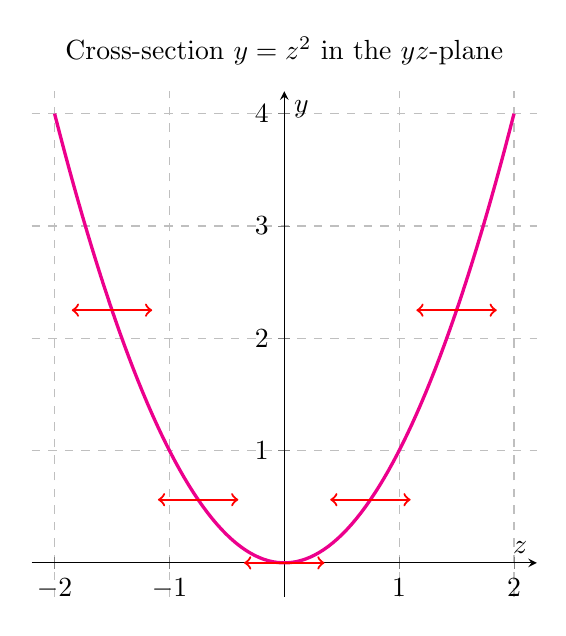
\begin{tikzpicture}
\begin{axis}[
    xlabel=$z$, ylabel=$y$,
    xmin=-2.2, xmax=2.2,
    ymin=-0.3, ymax=4.2,
    title={Cross-section $y=z^2$ in the $yz$-plane},
    width=8cm, height=8cm,
    axis lines=middle,
    grid=both,
    grid style={dashed, gray!50},
]
\addplot[magenta, very thick, domain=-2:2, samples=100] {x^2};
\addplot[red, ->, thick, domain=0:0.35] ({-1.5+x},{2.25});
\addplot[red, ->, thick, domain=0:0.35] ({-1.5-x},{2.25});
\addplot[red, ->, thick, domain=0:0.35] ({-0.75+x},{0.5625});
\addplot[red, ->, thick, domain=0:0.35] ({-0.75-x},{0.5625});
\addplot[red, ->, thick, domain=0:0.35] ({0+x},{0});
\addplot[red, ->, thick, domain=0:0.35] ({0-x},{0});
\addplot[red, ->, thick, domain=0:0.35] ({0.75+x},{0.5625});
\addplot[red, ->, thick, domain=0:0.35] ({0.75-x},{0.5625});
\addplot[red, ->, thick, domain=0:0.35] ({1.5+x},{2.25});
\addplot[red, ->, thick, domain=0:0.35] ({1.5-x},{2.25});
\end{axis}
\end{tikzpicture}
\end{document}